\section{Introduction}
\section{Tools}
\subsection{IDE}
Visual Studio Code was used for this project 

Used it before and will likely contiunue using it 
excellent support for a huge range of languages

\subsection{Version Control}
Some defintion
Useful for creating branches for experimental features
allowed working between different computers with ease
backups
\subsection{Database Visualisation}
Neo4j has several tools included as part of auraDB
Bloom is used to visualise the data as a graph, as discussed in the design section
Explore (or whatever it is called), is useful for testing queries quickly
\subsection{Libraries}
\subsection{Client Side}
cytoscape - used to create graphs on the front end
% rxjs?
material - googles own library of components to make ui quickly
\subsection{Server Side}
% neomodel
% more ...
\section{Data Processing}
this section covers getting the data needed to create the database and creating the database
\subsection{Finding Data Source}
fandom wikis all should have an xml dump available on the special:statistics page
It isnt always up to date, so i had to request a update
while waiting for that I looked at other BOI sources such as platinum god and the game files

got the xml file and its massive and not consistently formatted
it's set up like a huge list of pages but theres not order to them and sometimes random stuff is added in between them
looked challenging to extract data from so looked towards other games i.e. pokemon
however that wiki didn't have a dump at all and i got no response regarding getting one
other data sources for pokemon exist but each have their own issues
\subsection{Data Extraction}
while looking for alternative sources and waiting on response from wiki admins worked on extracting the data
used beautifulsoup to parse the xml tags and traverse the data
Used the items collection page to get the names of all the items locate the correct xml elements
trinkets and characters(?) had to be hardcoded as a complete list didnt exist in the xml

beautifulsoup is used to traverse the data and get the 'text' child of all the relevant 'pages'
then regex is used to grab the relevant sections from the text
\subsection{Cleaning the Data}
regex is used again to clean the sections of text
The text contains lots of tags for vairous features in the wiki such as dlc tags and links to other pages

\subsection{Importing into Database}
% generating CSV files in the correct format to use the data importer tool
\begin{figure}[H]
    \centering
    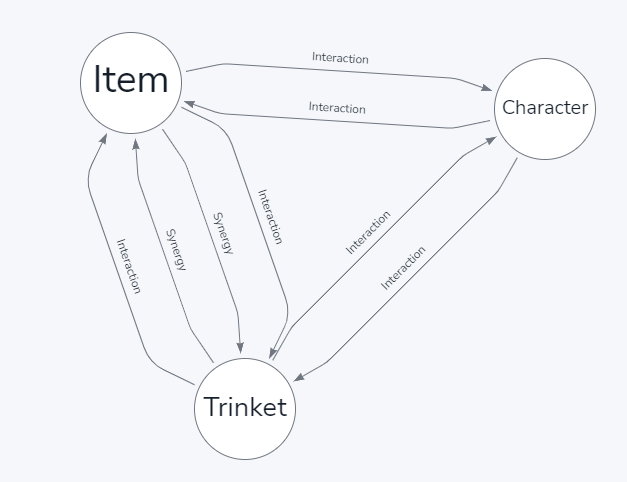
\includegraphics[scale=0.4]{dataImport}
    \caption{Database Model in Neo4j Data Importer}
\end{figure}
\section{Web Stack}
% creating the Django and angular projects and connecting them together
% talk about submodules
\section{Database Interaction}
% creating models
% finding cypher query for getting relationships and all data
% explain that it's really slow
\section{Client Side}
% tables
% using cytoscape to create graphs
% hardcoding files
\section{Conclusion}